\documentclass[12pt]{article}
\usepackage[T1]{fontenc}
\usepackage{calc}
\usepackage{setspace}
\usepackage{multicol}
\usepackage{fancyheadings}

\usepackage{graphicx}
\usepackage{color}
\usepackage{rotating}
\usepackage{harvard}
\usepackage{aer}
\usepackage{aertt}
\usepackage{verbatim}

\setlength{\voffset}{0in}
\setlength{\topmargin}{0pt}
\setlength{\hoffset}{0pt}
\setlength{\oddsidemargin}{0pt}
\setlength{\headheight}{0pt}
\setlength{\headsep}{.4in}
\setlength{\marginparsep}{0pt}
\setlength{\marginparwidth}{0pt}
\setlength{\marginparpush}{0pt}
\setlength{\footskip}{.1in}
\setlength{\textwidth}{6.5in}
\setlength{\textheight}{8.5in}
\setlength{\parskip}{0pc}

\renewcommand{\baselinestretch}{1.5}

\newcommand{\bi}{\begin{itemize}}
\newcommand{\ei}{\end{itemize}}
\newcommand{\be}{\begin{enumerate}}
\newcommand{\ee}{\end{enumerate}}
\newcommand{\bd}{\begin{description}}
\newcommand{\ed}{\end{description}}
\newcommand{\prbf}[1]{\textbf{#1}}
\newcommand{\prit}[1]{\textit{#1}}
\newcommand{\beq}{\begin{equation}}
\newcommand{\eeq}{\end{equation}}
\newcommand{\beqa}{\begin{eqnarray}}
\newcommand{\eeqa}{\end{eqnarray}}
\newcommand{\bdm}{\begin{displaymath}}
\newcommand{\edm}{\end{displaymath}}
\newcommand{\script}[1]{\begin{cal}#1\end{cal}}
\newcommand{\citee}[1]{\citename{#1} (\citeyear{#1})}
\newcommand{\h}[1]{\hat{#1}}
\newcommand{\ds}{\displaystyle}

\newcommand{\app}
{
\appendix
}

\newcommand{\appsection}[1]
{
\let\oldthesection\thesection
\renewcommand{\thesection}{Appendix \oldthesection}
\section{#1}\let\thesection\oldthesection
\renewcommand{\theequation}{\thesection\arabic{equation}}
\setcounter{equation}{0}
}

\pagestyle{fancyplain}
\lhead{}
\chead{Regime Switching, Learning, and the Great Moderation}
\rhead{\thepage}
\lfoot{}
\cfoot{}
\rfoot{}

\begin{document}

\begin{comment}
\begin{titlepage}
\begin{singlespace}
\title{Regime Switching, Learning, and the Great Moderation\footnote{I am grateful for the advice and guidance of Eric Leeper, Kim Huynh, Brian Peterson, and Todd Walker; for useful conversations with Fabio Milani and Bruce Preston; and for comments by the participants of Indiana University economics department seminars.  All errors are my own.}}
\date{September 30, 2008}
\author{James Murray\\
Dahl School of Business\\
Viterbo University\footnote{\textit{Mailing address}: 900 Viterbo Drive, La Crosse, WI  54601. \textit{E-mail address}: jmmurray@viterbo.edu.  \textit{Phone number}: (608)738-5408. }}

\maketitle

\thispagestyle{empty}

\abstract{This paper examines the ``bad luck'' explanation for changing volatility in U.S. inflation and output when agents do not have rational expectations, but instead form expectations through least squares learning with an endogenously changing learning gain.  It has been suggested that this type of learning can create periods of excess volatility without the need for exogenous changes in volatility.  Bad luck is modeled into a standard New Keynesian model by augmenting it with two states that evolve according to a Markov chain, where one state is characterized by large variances for structural shocks, and the other state has relatively smaller variances.  The model is estimated by maximum likelihood, and the results show that learning does lead to lower variances for the shocks in the volatile regime, but changes in regime is still significant in explaining the change in volatility occuring at the onset of the Great Moderation.
} \newline  

\noindent \textit{Keywords}: Learning, regime switching, great moderation, New Keynesian model, maximum likelihood. \\
\noindent \textit{JEL classification}: C13, E31, E50.
\end{singlespace}
\end{titlepage}
\newpage
\end{comment}


\section{Introduction}
Figure \ref{fg3:data} shows plots of the U.S. output gap, the percentage difference between the actual level of real GDP and potential GDP, and the inflation rate, as measured by the annualized quarterly growth rate of the consumer price index.  Aside from standard business cycle fluctuations, the data exhibits prolonged periods of differing degrees of volatility.  Output and inflation are especially volatile during the 1970s and early 1980s, and there has been a subsequent decline in volatility since that period.  \citee{kimnelson1999} estimate that since the first quarter of 1984, there has been a permanently smaller difference between the growth rate of output during expansions and during recessions.

Macroeconomics has had difficulty explaining this ``Great Moderation'', as it has come to be called.  The leading explanations for the change in volatility fall into two groups: good vs. bad monetary policy, and good vs. bad luck.  Using a standard New Keynesian model, \citee{ls2004} find empirical evidence of a change in monetary policy from bad to good, occurring sometime between 1979 and 1982.  They find that prior to 1979, the Federal Reserve did not adjust the federal funds rate by more than one-to-one with inflation, and therefore under rational expectations, the equilibrium was indeterminate and the economy was subject to sunspot shocks which led to greater volatility.  

Many studies find that a change in monetary policy is not enough to explain the change in volatility. \citee{simszha2006} find that evidence that changes in U.S. volatility is better explained by changes in luck than changes in monetary policy.  Using a structural vector autoregression model with minimal identification restrictions so that it can possibly encompass many sorts of linear dynamic macroeconomic models with a monetary policy rule, they find the best fitting model is one in which there are no regime changes in the coefficients describing monetary policy or economic behavior, and there are only regime changes in the variance of the exogenous shocks.  \citee{stockwatson2003} similarly find that improved monetary policy accounts for only a small part of the slowdown in macroeconomic volatility since 1984.

A third explanation that is just recently receiving some attention in the literature is that expectations that evolve according to least squares learning can lead to changing periods of volatility.  Under least squares learning, agents do not know the parameters that govern the economy.  Not being able to form rational expectations, they estimate least squares autoregressions using past data, and use this econometric model to forecast future variables.  \citee{milani2005} estimates a New Keynesian model with least squares learning and when splitting the sample at the same dates as \citee{ls2004}, finds there is little evidence of a change in monetary policy and estimates the federal funds rate did adjust by more than one-to-one with inflation throughout the sample.  

\citee{primiceri2006} demonstrates how learning on the part of the central bank can be perceived as bad monetary policy.  In an empirically founded model of unemployment rate and inflation determination he shows how mis-perceptions by the central bank about the natural rate of unemployment and the degree of persistence of inflation led to a bad policy prescription during the 1970s, and therefore excessively volatile unemployment and inflation.  As time progressed and more data became available, the Federal Reserve learned its mistakes and eventually provided better policy, leading to a slowdown in macroeconomic volatility after the mid-1980s.  \citee{stockwatson2003} provide some evidence for such an explanation when they demonstrate that univariate least squares forecasts have been more precise during less volatile periods.

Unlike previous papers in the learning literature, this paper estimates a model that combines the bad luck explanation along with learning to determine whether learning leads to a different prediction on the amount of bad luck needed to generate the changes in volatility seen in U.S. data.  Previous papers in the learning literature have allowed volatility to be affected only by learning dynamics, so it is not clear whether these explanations trump the bad luck explanation.  Changes in luck is modeled by assuming the variances of exogenous structural shocks are determined by a regime switching process with two states.  One state is characterized by large variances of the shocks and the other has relatively smaller variances.  Being in the volatile state is considered ``bad luck'' as the states evolve exogenously according to a Markov chain were the current state is only dependent on the previous state, and the probabilities of switching between states is exogenous.  

Agents do not have rational expectations, and are therefore completely unaware of any regime switching processes.  Agents do remain suspect that structural changes may occur, but they do not have any knowledge about what types of structural changes are possible, or any idea with what probabilities structural changes can occur.  Expectations therefore evolve according to a process similar to the \citee{marcetnicolini2003} framework where the weight agents give to older observations is endogenous.  Specifically, agents begin using a decreasing learning gain which consistent with forming ordinary least squares forecasts and having no suspicion of structural change.  If recent forecast errors become larger than the historical average, agents then suspect a structural change may have occurred and therefore increase their learning gain, giving larger weight to current observations which are believed to have more likely occurred after a structural break.

While a constant learning gain is theoretically capable of producing time varying volatility, in \citee{murray2008} I show in a New Keynesian model with no regime changes that constant gain learning is not able to deliver dynamics of U.S. inflation and output much better than rational expectations, and both frameworks especially fail to explain the excess volatility of the 1970s.  \citee{milani2007} simulates a model using parameters estimated with U.S. data that includes the endogenously changing learning gain similar to that suggested by \citee{marcetnicolini2003} and finds that this type of learning can produce heteroskedasticity in output and inflation that rational expectations simulations cannot.  Moreover, his estimates imply that during most of the 1970s decade, agents suspected structural change and therefore used a high learning gain.  

This paper builds on Milani's analysis by also allowing for recurrent regime changes in the volatility of the structural shocks.  Estimation of this model decomposes the changes in volatility into changes in the volatility of structural shocks and endogenous changes in the learning gain.  The main finding is that learning indeed leads to much smaller variances of structural shocks in the volatile regime.  However, changes in regime are still significant and the learning frameworks and rational expectations framework make similar predictions for the periods in U.S. history when the economy was in the volatile regime.  Despite the ability for learning to explain much of the volatility, the change in the dynamic gain appears to play an insignificant role, and the rational expectations model dominates the learning models in terms of its fit to the data.

The paper proceeds as follows. Section 2 presents the New Keynesian framework and regime switching process.  Section 3 describes the learning process and how constant gain learning and dynamic gain learning can generate time varying volatility.  Section 4 describes the data and estimation procedure.  Section 5 presents the estimation results and interprets the findings, and Section 6 concludes.

\section{Model}
The crucial extensions of learning with an endogenously changing gain and a Markov chain process for changes in volatility are incorporated into a standard New Keynesian model of output and inflation determination and monetary policy.  This section describes the rational expectations version New Keynesian model and the next section introduces learning in the linearized version of the model.\footnote{This methodology is perhaps the most common means for putting learning into macroeconomic models, but \citee{preston2005} demonstrates that since the least squares expectations operator does not follow the law of iterated expectations, this method is not consistent with learning inherent in the microfoundations of the model.}

There are a continuum of consumers types on the unit interval, and a continuum of intermediate goods producers on the same unit interval.  Each consumer type has a specific labor skill that is only hired by the corresponding intermediate goods producer.  It is assumed there are a number of consumers of each type, so that no consumer has market power over the wage, and that there are an equal number of consumers in each type, so that relative output levels of intermediate goods do not depend on the distribution of consumer types.

There is one final good that is used for consumption, and produced using all the intermediate goods.  The intermediate goods are imperfect substitutes for each other in production, therefore intermediate goods firms are monopolistically competitive.  Prices for intermediate goods are subject to a \citee{calvo1983} pricing friction where only a fraction of firms are able to re-optimize their price every period, and the firms fortunate to do so is randomly determined, independently of firms' histories.

\subsection{Consumers}
Each consumer type has a specific labor skill that can only be hired by a specific intermediate goods producing firm.  Since each intermediate goods firm has a different labor demand, wage income will be different for each consumer type.  However, given a perfect asset market, consumption will be equal across all consumers.  Each consumer type $i \in (0,1)$ maximizes utility,
\bdm E_0 \sum_{t=0}^{\infty} \beta^t \left[ \frac{1}{1-\frac{1}{\sigma}} \xi_t \left(c_t - \eta c_{t-1}\right)^{1-\frac{1}{\sigma}} - \frac{1}{1+\frac{1}{\mu}} n_t(i)^{1+\frac{1}{\mu}} \right], \edm
subject to the budget constraint,
\bdm c_t + b_t(i) = \frac{1+r_{t-1}}{1+\pi_t} b_{t-1}(i) + \frac{w_t(i)}{p_t} n_t(i) + \Pi_t - \tau_t. \edm
Consumption at time $t$, given by $c_t$, is not indexed by individual type $i$ since it is equal across all agents.  The remaining variables include $\xi_t$, which is an aggregate preference shock, $n_t(i)$ and $w_t(i)/p_t$ are the labor supply and real wage of individual $i$ at time $t$, respectively, $b_t(i)$ is individual $i$'s purchase of real government bonds at time $t$, $r_t$ is the nominal interest rate paid on government bonds, $\pi_t$ is the inflation rate of the price of the final good, $\Pi_t$ is the value of profits earned by owning stock in firms, and $\tau_t$ is the value of real lump sum taxes.  The preference parameters are $\sigma \in (0,\infty)$, which is the intertemporal elasticity of substitution, $\mu \in (0,\infty)$, which is the elasticity of labor supply, and $\eta \in [0,1)$, which is the degree of habit formation.  

Habit formation is added to the model because it introduces a source of consumption (and therefore output) persistence that has been found to be significant in rational expectations models.  For example, \citee{smetswouters2005} estimate a rational expectations New Keynesian model with numerous extensions for both the United States and Euro area and find point estimates for the degree of habit formation very close to unity.  Furthermore, \citee{fuhrer2000} finds that habit formation leads to ``hump shaped'' impulse response functions that can be supported by the data.  The importance of habit formation may not be so important when dropping the assumption of rational expectations.  \citee{milani2005} shows that under learning the estimate for the degree of habit formation falls close to zero.

Log-linearizing the consumers' first order conditions leads to the following Euler equation,
\beq \label{eq3:lneuler} \h{\lambda}_{t} = E_t \h{\lambda}_{t+1} + \h{r}_t - E_t \pi_{t+1}, \eeq
where a hat indicates the percentage deviation of the variable from its steady state.\footnote{A hat is omitted from inflation because it will be necessary to assume the steady state inflation rate is equal to zero when log-linearizing the firms' profit maximizing conditions.}  Here, $\h{\lambda}_t$ is the marginal utility of real income, given by,
\beq \label{eq3:lnlambda} \h{\lambda}_t = \frac{1}{ (1-\beta \eta)(1-\eta)}\left[ \beta \eta \sigma E_t \h{c}_{t+1} - \sigma(1+\beta \eta^2) \h{c}_t + \sigma \eta \h{c}_{t-1} \right] + \left(\h{\xi}_t - \beta \eta E_t \h{\xi}_{t+1} \right). \eeq

\subsection{Production}
There is one final good used for consumption and investment which is sold in a perfectly competitive market and produced with a continuum of intermediate goods.  The production function is given by,
\beq \label{eq3:yprod} y_t = \left[ \int_0^1 y_t(i)^{\frac{\theta-1}{\theta}} di \right]^{\frac{\theta}{\theta-1}}, \eeq
where $y_t$ is the output of the final good, $y_t(i)$ is intermediate good $i$, and $\theta \in (1,\infty)$ is the elasticity of substitution in production.  Profit maximization leads to the demand for each intermediate good,
\beq \label{eq3:yi} y_t(i) = \left[ \frac{p_t(i)}{p_t} \right]^{-\theta} y_t, \eeq
where $p_t(i)$ is the price of intermediate good $i$ and $p_t$ is the price of the final good.  Substituting equation (\ref{eq3:yi}) into (\ref{eq3:yprod}) leads to a consumption price index that holds in equilibrium,
\beq \label{eq3:pfinal} p_t = \left[ \int_0^1 p_t(i)^{1-\theta} di \right]^{\frac{1}{1-\theta}}. \eeq

Each intermediate good is produced according the constant returns to scale production function $y_t(i) = \zeta_t n_t(i)$, where $\zeta_t$ is an exogenous technology shock common to all firms.  Given a level of production $y_t(i)$, firms choose labor demand to minimize total cost $\frac{w_t(i)}{p_t}n_t(i)$.  When labor markets clear, it can be shown that firm $i$'s optimal choice for labor leads to the log-linearized marginal cost of firm $i$ equal to,
\beq \label{eq3:mc} \h{\psi}_t(i) = \frac{1}{\mu} \h{y}_t(i) - \h{\lambda}_t - \left(\frac{1}{\mu} + 1\right) \h{\zeta}_t. \eeq
Summing equation (\ref{eq3:mc}) across all firms leads to the average marginal cost in the economy,
\beq \label{eq3:mc2} \h{\psi}_t = \frac{1}{\mu} \h{y}_t - \h{\lambda}_t - \left(\frac{1}{\mu} + 1\right) \h{\zeta}_t. \eeq

Firms' pricing decisions are subject to the \citee{calvo1983} pricing friction, where only a constant fraction of firms are able to re-optimize their in a given period.  I suppose that firms who are not able to re-optimize their price may adjust their price by a fraction, $\gamma$, of the previous period's inflation rate.  Let $\omega \in (0,1)$ denote the fraction of firms who are not able to re-optimize their prices each period.  Since these specific firms are randomly determined, $\omega^T$ is the probability a firm will not be able to re-optimize its price for $T$ consecutive periods.  A firm who is able to re-optimize its price maximizes the following present discounted utility value of profits earned while the firm is unable to re-optimize its price again:
\beq \label{eq3:intprofit}
E_t \sum_{T=0}^{\infty} \left(\omega \beta \right)^{T} \frac{\lambda_{t+T}}{\lambda_t}
\left\{ \left(\frac{p_{t}(i) \pi_{t+T}^{*}}{p_{t+T}}\right) y_{t+T}(i) - \Psi\left[y_{t+T}(i)\right] \right\},
\eeq
where $\Psi\left[y_{t+T}(i)\right]$ is the real total cost function of producing $y_{t+T}(i)$ units, given the optimal decision for labor, and $\pi_{t+T}^{*} = \prod_{j=1}^{T} (1+\gamma \pi_{t+j-1})$ is degree to which the firm's price is able to adjust according to inflation indexation.  It can be shown that the first order condition for $p_{t}(i)$ combined with the final good price index, equation (\ref{eq3:pfinal}), leads to the log-linear Phillips equation,
\beq \label{eq3:phillips} \pi_t = \frac{1}{1+\beta \gamma} \left[ \gamma \pi_{t-1} + \beta E_t \pi_{t+1} + \frac{\mu (1-\omega)(1-\omega \beta)}{\omega (\mu + \theta)} \h{\psi}_t \right] \eeq

\subsection{Fully Flexible Prices}
To take this model to data on the output gap it is convenient to rewrite the model in terms of the difference from the outcome in which there are no nominal rigidities.  Let $\tilde{y}_t = \h{y}_t - \h{y}_t^f$ and $\tilde{\lambda}_t = \h{\lambda}_t - \h{\lambda}_t^f$ denote the percentage deviation of output and marginal utility from their fully flexible price outcome.  Under fully flexible prices the linearized Euler equation, (\ref{eq3:lneuler}), and marginal utility of income, (\ref{eq3:lnlambda}), still hold.  Using these conditions and imposing goods market equilibrium condition implies,
\beq \label{eq3:gapeuler} \tilde{\lambda}_{t} = E_t \tilde{\lambda}_{t+1} + \h{r}_t - E_t \pi_{t+1} - r_t^n, \eeq
\beq \label{eq3:gaplambda} \tilde{\lambda}_t = \frac{1}{ (1-\beta \eta)(1-\eta)}\left[ \beta \eta \sigma E_t \tilde{y}_{t+1} - \sigma(1+\beta \eta^2) \tilde{y}_t + \sigma \eta \tilde{y}_{t-1} \right], \eeq
where $r_t^n$ is the percentage deviation of natural interest rate from its steady state.  The ``natural interest rate'' is the interest rate that would occur under fully flexible prices.  I suppose that $r_t^n$ follows the stochastic exogenous process,
\beq \label{eq3:natint} r_t^n = \rho_n r_{t-1}^n + \epsilon_{n,t}, \eeq
where $\epsilon_{n,t}$ is an independently and identically distributed shock.

When prices are fully flexible, $\omega=0$ in the maximization problem given in equation (\ref{eq3:intprofit}).  It can be shown in this case that the first order condition implies the marginal cost is identical for every firm and always constant. Under fully flexible prices equation (\ref{eq3:mc2}) implies,
\bdm \h{\psi}_t^f = 0  = \frac{1}{\mu} \h{y}_t^f - \h{\lambda}_t^f - \left(\frac{1}{\mu} + 1\right) \h{\zeta}_t. \edm
One can solve this equation for $\h{\zeta}_t$ and substitute that back into the equation for marginal cost (\ref{eq3:mc2}).  Plugging this expression for marginal cost into equation (\ref{eq3:phillips}) yields the following Phillips curve in terms of the output gap,
\beq \label{eq3:phillips1} \pi_t = \frac{1}{1+\beta \gamma} \left[ \gamma \pi_{t-1} + \beta E_t \pi_{t+1} + \frac{(1-\omega)(1-\omega \beta)}{\omega (\mu + \theta)} (\tilde{y}_t - \mu \tilde{\lambda}_t) \right]. \eeq
While this expression for the Phillips curve is not subject to a structural shock, when estimating the model by maximum likelihood it is convenient to have a shock here to avoid the problem of stochastic singularity.  The Phillips curve is amended with a ``cost-push'' shock so the form that is estimated is given by,
\beq \label{eq3:gapphillips} \pi_t = \frac{1}{1+\beta \gamma} \left[ \gamma \pi_{t-1} + \beta E_t \pi_{t+1} + \kappa (\tilde{y}_t - \mu \tilde{\lambda}_t) + u_t\right], \eeq
where $\kappa$ is the reduced form coefficient on the marginal cost and $u_t$ is an exogenous cost-push shock that evolves according to,
\beq \label{eq3:costpush} u_t = \rho_u u_{t-1} + \epsilon_{u,t}, \eeq
where $\epsilon_{u,t}$ is an independently and identically distributed shock.

\subsection{Monetary Policy}
The nominal interest rate is determined jointly with output and inflation by monetary policy.  In this paper I assume the monetary authority follows a \citee{taylor1993} type rule of the form,
\beq \label{eq3:taylor} \h{r}_t = \rho_r \h{r}_{t-1} + (1-\rho_r) \left(\psi_{\pi} E_t \pi_{t+1} + \psi_y E_t \tilde{y}_{t+1} \right) + \epsilon_{r,t} \eeq
where $\rho_r \in [0,1)$ is a degree of interest rate smoothing desired by the monetary authority, $\psi_{\pi} \in (0,\infty)$ is the feedback on the interest rate to expected inflation, $\psi_y \in (0,\infty)$ is the feedback on the interest rate to the expected output gap, and $\epsilon_{r,t}$ is an independently and identically distributed exogenous monetary policy shock.

\subsection{Regime Switching}
The bad luck explanation for why the United States experienced periods of excessive volatility is that the variances of the structural shocks were larger during these periods.  To model this explanation in the framework of the New Keynesian model I suppose the variance of the natural interest rate shock $\epsilon_{n,t}$, the cost push shock, $\epsilon_{u,t}$, and the monetary policy shock $\epsilon_{r,t}$  are determined by two states.  Let state $L$, denoted by $s_L$, be the state where the shocks have low volatility, and state $H$, denoted by $s_H$, be the state where the shocks have high volatility. 

The variances of the structural innovations in a given state are independently normally distributed with mean zero and variances given by,
\beq \label{eq3:vars}
Var\left[ \epsilon_t(s_t) \right] = \left\{
 \begin{array}{c} \left[ \begin{array}{ccc} \sigma_{n,L}^2 & 0 & 0 \\ 0 & \sigma_{u,L}^2 & 0 \\ 0 & 0 & \sigma_{r,L}^2 \end{array} \right], \mbox{       if $s_t=L$} \\ 
\left[ \begin{array}{ccc} \sigma_{n,H}^2 & 0 & 0 \\ 0 & \sigma_{u,H}^2 & 0 \\ 0 & 0 & \sigma_{r,H}^2 \end{array} \right], \mbox{       if $s_t=H$} 
\end{array} \right\}, \eeq
where $\epsilon_t(s_t)' = \left[ \epsilon_{n,t}(s_t) ~ \epsilon_{u,t}(s_t) ~ \epsilon_{r,t}(s_t) \right]$, and the variances in the high volatility state are greater than or equal to the variances in the low volatility state.  

The state $s_t$ evolves according to a two state Markov chain.  Let $p_j \in (0,1)$ denote the probability of staying in state $j$ at time $t$, given the economy is at state $j$ at time $t-1$, for $j \in \{L,H\}$.  This implies that the probability of moving from state $i$ in $t-1$ to state $j$ in time $t$, where $i\neq j$ is given by $1-p_j$ .  The state then evolves according to the transition matrix,
\beq \label{eq3:tran} P = \left[ \begin{array}{cc} p_L & 1-p_L \\ 1-p_H & p_H \end{array} \right]. \eeq
Let $S_t' = [P(s_t=L)~ P(s_t=H)]$ denote the probability of being in each state at any given time $t$.  The transition matrix assumes the state evolves according to,
\beq \label{eq3:tranevo} E_t S_{t+1} = P S_{t} \eeq

Notice this regime switching framework makes the somewhat restrictive assumption that all structural shocks are always in the same regime.  A less restrictive assumption would be that one or more shocks could be in one regime while one or more others could be in another regime.  Such a setup would require specifying a transition matrix for each structural shock.  If one assumed that the different shocks transitioned between regimes independently of one another, this would introduce four more parameters to be estimated.  If one wanted to generalize the process so that there is some dependence, this would involve even more parameters.  To keep the number of parameters to estimate tractable, and to avoid over-fitting the data, I assume that all shocks are in the same regime in a given time period.

\section{Learning}
Instead of having rational expectations, agents form expectations by estimating least squares regression models, where expectations of future output and inflation are given by the forecasts from these models.  Agents are assumed to have no knowledge of the structural form of the economy, the parameters that govern the economy, or the regime switching process.  They do know the reduced form of the economy follows a VAR(1) process, and they use this model and past data to form their forecasts. 

The model in the previous section only allows for structural changes in the volatility in the shocks, and since the model is linearized, agents are indifferent to the additional risk.  Even so, I suppose that agents suspect that structural changes of unknown types are possible so they may decide to give more weight to recent observations in their estimation procedure.  One way to model this is to use constant gain learning, which is consistent with agents using forecasts based on weighted least squares estimates, where the weights decline geometrically with the age of the observations.  With a constant gain, the weight put on the latest observation is always the same, regardless of how much data the agents already have for their forecasts.  One benefit of this type of learning is that learning dynamics persist in the long run.  

Authors such as \citee{sargent1999} and \citee{evanshonka2001} have suggested that constant gain learning is a natural way to model expectations in a real world where structural changes, perhaps large or small, are always possible.  The drawback of constant gain learning is that it implies agents always have the same level of suspicion for structural changes, regardless of recent macroeconomic activity or the size of recent forecast errors.  If agents instead use ordinary least squares (OLS), then the weight agents give to additional observations diminishes as their sample size approaches infinity.  Said another way, the learning gain decreases and approaches zero as time approaches infinity, causing learning dynamics to disappear completely in the long run.  Learning with OLS also implies that agents believe structural changes that should impact their decisions are impossible.

Constant gain learning can in theory lead to time varying volatility of expectations, and therefore time varying volatility for output and inflation.  This affect depends on the size of the constant learning gain, but for empirically plausible values, this type of learning fails to deliver very big effects.   \citee{williams2003} finds this to be the case in a simple model with simulated data. 

\citee{marcetnicolini2003} suggest an alternative way to model dynamic expectations.  Instead of assuming that agents never suspect a structural change, as is consistent with OLS, or assuming that agents always suspect a structural change with equal likelihood, as is consistent with a constant gain, they take a mixture of these methods where the learning gain changes endogenously.  Suppose agents begin with no suspicion of recent structural changes.  As time progresses they form their expectations using a decreasing learning gain consistent with OLS.  Agents will suspect a structural change may have occurred if recent forecast errors are larger than historical averages.  When this happens, agents switch to a larger learning gain, which puts more weight on the most recent observations, ones that are believed to have more likely occurred after a structural change.  As long as forecast errors are large, the learning gain remains at this high point.  When forecast errors start becoming small, the learning gain decreases at a rate consistent with OLS.  I explain in more detail the endogenous learning gain process below, but first it is first necessary to explain specific details of least squares learning in the framework of a dynamic stochastic general equilibrium model like the New Keynesian model in Section 2.

\subsection{Least Squares Learning}
The log-linearized model in Section 2 can be expressed in the general form:
\beq \label{eq3:sform} \Omega_{0} x_t = \Omega_{1} x_{t-1} + \Omega_{2} E_t^* x_{t+1} + \Psi z_t, \eeq
\beq \label{eq3:sformsh} z_t = A z_{t-1} + \epsilon_t(s_t) \eeq
where $E_t^*$ denotes possibly non-rational expectations, $x_t$ is a vector of minimum state variables, and $z_t$ is a vector of structural shocks.  For the New Keynesian model, $x_t = [\tilde{y}_t~ \pi_t~ \h{r}_t~ \tilde{\lambda}_t]'$ and $z_t = [r_t^n~ u_t~ \epsilon_{r,t}]'$.  The minimum state variable solution of the model implies the rational expectation for $x_{t+1}$ is given by,
\beq \label{eq3:msvsol} E_t x_{t+1} = G x_{t} + H E_t z_{t+1}, \eeq
where the elements of the matrices $G$ and $H$ are a function of the parameters of the model and may be determined by the method of undetermined coefficients.  Agents that learn do not know the the parameters that govern the economy, but do use the reduced form of the economy for their forecasting model.  Agents' information sets are restricted only to past data on $x_t$, so they are unable to collect data on past structural shocks to estimate matrix $H$.  Therefore, agents collect past data on $x_t$ to form least squares estimates for the non-zero columns of $G$.

Agents do know what columns of $G$ are equal to zero, and therefore do not use the associated variables as explanatory variables in their regression.  In terms of the New Keynesian model in the previous section, the only non-zero column of $G$ is that which multiplies past marginal utility of income, $\tilde{\lambda}_t$.  When there is a positive degree of habit formation, not only are expectations of next period's output important for consumers' decisions, so is next period's future marginal utility of income which involves a two period ahead forecast for output.  Since the only sources of persistence in the model are on output (habit formation), inflation (price indexation), and the interest rate (monetary policy smoothing), these are the only variables whose lags agents use as explanatory variables.  

The timing in which agents make expectations and decisions in a given period is as follows.  At the beginning of period $t$ agents wake up with data realized through period $t-1$.  They collect this data and use the least squares estimate for $G$ to make forecasts for future realizations of variables such as output and inflation.  Given these expectations, agents consumption and pricing decisions are implemented and only then do time $t$ outcomes become realized.  In the next period, these outcomes become available as data to the agents, and the process begins again.  

There is no constant term in the general form of the model, equation (\ref{eq3:sform}), or in the rational expectation, given in equation (\ref{eq3:msvsol}), since all variables are expressed in terms of percentage deviations from the steady state or flexible price outcome.  Since agents are not endowed with information about the parameters of the model, it is realistic to suppose that agents also estimate a constant term in equation (\ref{eq3:msvsol}).  Let $\h{G}_t^*$ denote agents' time $t$ estimate for the non-zero columns of matrix $G$ and a column for a constant term so that $\h{G}_t^* = [\h{g}_{t}~ \h{G}_t^{NZ}]$, where $\h{g}_{t}$ is the time $t$ estimate of the constant term and $\h{G}_t^{NZ}$ is the time $t$ estimate for the non-zero columns of $G$. 

If agents use OLS, then,
\beq \label{eq3:Gsum} \left(\hat{G}_t^*\right)' = \left( \frac{1}{t-1} \sum_{\tau=1}^{t-1} x_{\tau-1}^* {x_{\tau-1}^{*}}' \right)^{-1} \left( \frac{1}{t-1} \sum_{\tau=1}^{t-1} x_{\tau-1}^* x_{\tau}' \right), \eeq 
where $x_t^{*'} = [1~ x_t^{NZ'}]$ is the vector of explanatory variables agents use.   Agents form the expectation,
\beq \label{eq3:agfore} E_t^* x_{t+1} = \h{g}_{t} + \h{G}_t E_t^* x_t = (I + \h{G}_t)\h{g}_{0,t} + \h{G}_t^2 x_{t-1}, \eeq
where $\h{G}_t$ denotes the time $t$ estimate for $G$ obtained from $\h{G}_t^{*}$ with the zero columns filled back in.  The least squares estimate for $\h{G}_t^*$ can be rewritten in the following recursive form:
\beq \label{eq3:lnG} \hat{G}_t^* = \hat{G}_{t-1}^* + g_t (x_{t-1} - \hat{G}_{t-1}^* x_{t-2}^*) {x_{t-2}^*}' R_t^{-1} ,\eeq
\beq \label{eq3:lnR} R_t = R_{t-1} + g_t (x_{t-2}^* {x_{t-2}^*}' - R_{t-1}), \eeq
where $g_t=1/(t-1)$ is the learning gain.\footnote{To show this, let $R_t = \frac{1}{t-1} \sum_{\tau=1}^{t-1} x_{\tau-1}^* x_{\tau-1}^{*'}$ and $\left(\hat{G}_t^*\right)' = R_t^{-1} \left( \frac{1}{t-1} \sum_{\tau=1}^{t-1} x_{\tau-2}^* x_{\tau-1}' \right)$.}
The recursive form shows precisely how expectations are adaptive.  The term enclosed in parentheses in equation (\ref{eq3:lnG}) is the realized forecast error for the previous estimate $\hat{G}_{t-1}^*$.  The degree to which agents adjust their expectations depends on the size of this forecast error, the variance of the estimated coefficients, captured by the inverse of matrix $R_t$, and the size of the learning gain, $g_t$.  The larger is the learning gain, the more expectations respond to the latest forecast error.  When agents use OLS, $g_t$ approaches zero as time approaches infinity.  Under constant gain learning, $g_t$ remains at some constant level, $g$, so the degree to which new observations can affect expectations is always the same.  

Substituting the expectation in equation (\ref{eq3:agfore}) into the structural form, (\ref{eq3:sform}), leads to the following evolution for $x_t$,
\beq \label{eq3:evolx} x_t = \Omega_0^{-1} \Omega_2 (I+\h{G}_t) \h{g}_{0,t} + \Omega_0^{-1} \left( \Omega_1 + \Omega_2 \h{G}_t^2 \right) x_{t-1} + \Omega_0^{-1} \Psi z_t, \eeq
where $\h{g}_{0,t}$ and $\h{G}_t$ are determined by the learning process in equations (\ref{eq3:lnG}) and (\ref{eq3:lnR}).  

This form illustrates how learning with a positive learning gain can lead to time-varying volatility for $x_t$ even if with a constant variance for $z_t$.  Unlike standard rational expectations models, the constant term and matrix multiplying $x_{t-1}$ are time-varying.  The magnitude of these matrices depends on the size of the learning gain and the size of agents' forecast errors.  Time variation in these matrices causes time variation in the volatility of $x_t$.  Note this is true for any non-zero value for the learning gain $g_t$.  Even a constant learning gain can technically generate time-varying volatility, but time variation in the learning gain has been suggested by \citee{marcetnicolini2003} and \citee{milani2007} to better explain such phenomenon.

\subsection{Dynamic Gain Learning}
Under a mixed learning framework, the learning gain $g_t$ decreases over time, but may endogenously jump to a higher level when forecast errors are especially large.  Let $\alpha_t \equiv 1/g_t$ be the inverse of the learning gain, which under ordinary least squares is interpreted as the sample size.  The learning gain is assumed to evolve according to,
\beq \label{eq3:mngain} \alpha_t = \left\{ \begin{array}{cl} \ds \alpha_{t-1} + 1 & \ds \mbox{     if  } \frac{1}{J} \sum_{j=1}^{J} \frac{1}{n} \sum_{v=1}^{n} \left| x_{t-j}(v) - \hat{G}_{t-j}^*(v) x_{t-j-1}^* \right| < \nu_t \\
\ds \alpha & \ds \mbox{     otherwise} \end{array} \right\} \eeq
where $n$ denotes the number of variables in the model, $x_{t-j}(v)$ denotes the $v$th element of $x_{t-j}$ and $\hat{G}_{t-j}^*(v)$ denotes the $v$th row of $\hat{G}_{t-j}^*$, which is used to forecast variable $v$.  The parameter $J$ is the number of recent periods agents look at when deciding to change their learning gain.  \citee{marcetnicolini2003} assume $J=1$, so that agents may change their learning gain looking at only the most recent forecast error.  I fix $J=8$, so for quarterly data agents examine the forecast errors from the most recent two years and adjust the learning gain if the average forecast error during this time is too large.  The variable $\nu \in (0,\infty)$ is the threshold for how large the forecast errors must be to induce agents to increase their learning gain.  Similar to \citee{milani2007}, this threshold is set equal to the average size of forecast errors up through date $t-1$, which is given by,
\bdm \nu_t = \frac{1}{t-1} \sum_{j=1}^{t-1} \frac{1}{n} \sum_{v=1}^{n} \left| x_{t-j}(v) - \hat{G}_{t-j}^*(v) x_{t-j-1}^* \right|. \edm

 Since forecast errors for each variable $v$ is given as a percentage deviation from the steady state or potential, they are added up over all the variables that agents forecast.  This learning mechanism can nest the special cases when agents always use OLS or always use a constant gain.  To restrict agents to always use OLS, $\nu_t$ can be set to zero for all $t$.  To restrict agents to always use a constant gain, $\nu_t$ can be set to infinity for all $t$.

This learning mechanism introduces one additional parameter to estimate jointly with the parameters of the New Keynesian model and regime switching process, the threshold learning gain, $g \equiv 1/\alpha$.

\section{Estimation}
The model is estimated with quarterly U.S. data from 1960:Q1 through 2007:Q1 on the output gap, as measured by the Congressional Budget Office, the inflation rate of the consumer price index, and the Federal Funds rate.  The model conforms to a state-space representation with Markov-switching in the variance of the error term and is estimated using the \citee{kimnelson} technique for combining the Kalman filter that evaluates a state-space model with the \citee{hamilton1989} filter for evaluating Markov-switching processes.

\subsection{Maximum Likelihood Procedure}
The state side of the model is given by equations (\ref{eq3:evolx}) and (\ref{eq3:sformsh}).  Let $GAP_t$ denote data on the output gap, $INF_t$ denote data on inflation, and $FF_t$ denote data on the Federal Funds rate.  The observation equations are given by,
\bdm \begin{array}{c} \label{eq3:obs}  
\ds GAP_t = 100 \tilde{y}_t, \\
\ds INF_t = \pi^{*} + 400\pi_t, \\
\ds FF_t = r^{*} + \pi^* + 400\h{r}_t.
\end{array}
\edm
The state variables are multiplied by $100$ to convert the decimals into percentages, and the inflation rate and federal funds rate are multiplied by $4$ to convert the quarterly rates to annualized rates.  The New Keynesian model assumes that the steady state inflation rate is equal to zero, but since this is not likely the case in the data, the annualized steady state inflation rate, given by  $\pi^*$, is estimated along with the other parameters of the model.  The steady state gross real interest rate is set equal to the inverse of the discount factor; therefore $r^* = 400(1-1/\beta)$.

The log-likelihood is maximized with respect to the threshold learning gain, $g$, the Markov-switching probabilities, $p_h$ and $p_L$, the parameters of the New Keynesian model, and the variances of the structural shocks for each regime.  The discount factor is not estimated but instead fixed to $\beta=0.99$ which implies a steady state real interest rate of about 4\%.  The elasticity of substitution between intermediate goods, $\theta$, and the degree of price flexibility, $\omega$, appear multiplicatively in the Phillips curve (\ref{eq3:phillips1}) and so only the reduced form coefficient, $\kappa$, is estimated.  Before revealing the estimation results, it is first necessary to specify how initial conditions for the learning process are set.

\subsection{Initial Conditions}
Aside from standard initial conditions for the Kalman filter and Hamilton filter, it is necessary to specify initial conditions for the learning process given in equations (\ref{eq3:lnG}) and (\ref{eq3:lnR}).  How values are set for initial expectation matrices, $\h{g}_{0}$, $\h{G}_{0}^{*}$, and $R_{0}$, can have a dramatic effects on the estimation results.  Despite this dependence, there is little general consensus for how initial expectations should be specified.

\citee{williams2003} shows that using the rational expectations solution for initial expectations produces nearly identical dynamics as assuming expectations are rational throughout the sample.  Given the model is E-stable, this result is not too surprising.  If the conditions for E-stability are met, under a decreasing learning gain consistent with OLS, the model will converge to the rational expectations solution when in the neighborhood of this solution.  

Most initialization methods are therefore based on pre-sample evidence.  \citee{slobodyan_wouters2007} estimate the rational expectations version of the model on pre-sample data, and use the implied expectations as the initial condition for the sample.  \citeauthor{milani2005} (\citeyear{milani2005}, \citeyear{milani2007}) sets the initial conditions for the learning matrices equal to VAR(1) estimates from de-meaned pre-sample data.  Similarly, I estimate the appropriate regressions with pre-sample data from 1954:Q2 through 1959:Q4.  In the New Keynesian framework, agents estimate four regression models for the following dependent variables: output gap, inflation rate, interest rate, and marginal utility of income gap.  Each of these variables depends on lagged output gap, inflation rate, and interest rate.  The data must first be transformed into the same terms as the state vector, $x_t$.  For the output gap, inflation rate, and interest rate this is done according to:
\bdm \begin{array}{c}
\ds \tilde{y}_t = \frac{1}{100} GAP_t \\
\ds \pi_t = \frac{1}{400} (INF_t - \pi^{*}), \\
\ds \h{r}_t = \frac{1}{400} (FF_t - r^{*} - \pi^*).
\end{array}
\edm

Expectations for these first three variables in the state vector is found by estimating a VAR(1) on $[\tilde{y}_t~ \pi_t~ \h{r}_t]'$.  Data for the marginal utility of income gap is found by plugging into equation (\ref{eq3:gaplambda}) data for the output gap, lagged output gap, and expected future output gap predicted by the VAR(1).  Expectations for $\tilde{\lambda}_t$ are then found by regressing this simulated data on lagged $[\tilde{y}_t~ \pi_t~ \h{r}_t]'$.

\section{Results}
To analyze how learning and regime switching in volatility are related, the New Keynesian model is estimated under rational expectations, constant gain learning, and dynamic gain learning gain.  Table \ref{tb3:parms} presents the parameter estimates for each case.  Under constant gain learning, the estimate for learning gain is essentially equal to zero.  This implies that expectations do not evolve through the sample.  Even so, the predictions under constant gain learning are not the as same rational expectations, since the coefficient matrices agents use to form expectations are different.  The expectation matrices for the learning case are initialized to pre-sample VAR(1) results, which do not coincide with rational expectations.  The estimated threshold gain under dynamic gain learning has a very small point estimate, $g=0.0045$, but it is statistically significantly different from zero.  This implies that expectations do evolve over time, but the rate at which agents learn is very small.  

Comparing the standard deviation of the shock processes illustrates how expectations explain macroeconomic volatility.  There is little difference in the predictions for the volatility of the cost push and monetary policy shocks, but there is a substantial difference in the volatility for the natural rate shock.  For both the low and high volatility regime, the estimate for the variance of the natural rate shock under rational expectations is almost twice as high as under constant gain learning, and almost four times higher than under dynamic gain learning.  This implies that using the VAR(1) on pre-sample data to specify expectations explains much of the volatility in output, but evolving expectations with dynamic learning gain explains even more.  The persistence of the natural rate shock is also somewhat larger under rational expectations ($\rho_n=0.8705$), than under dynamic gain learning ($\rho_n=0.7484$) or constant gain learning ($\rho_n=0.6936$).  

Other parameter estimates that differ across models include the intertemporal elasticity of substitution and the Phillips curve slope.  The elasticity of substitution is approximately $\sigma=0.0073$ under rational expectations, $\sigma=0.2560$ under dynamic gain learning, and $\sigma=0.1824$ under constant gain learning.  This implies the intertemporal consumption trade-off is much more sensitive to the expected real interest rate with the initial expectations for the learning processes than under rational expectations.  Moreover, dynamic gain learning leads to an even higher estimate than the zero constant gain, although the difference is not statistically significant.

The estimates for the Phillips curve coefficient reveals how learning dynamics can alter the prediction for the degree of price flexibility.  The coefficients under rational expectations and constant gain learning are both very close to zero, which implies a very small degree of price flexibility.  However, under dynamic gain learning, the only framework in which expectations are evolving, the Phillips curve coefficient is much larger, implying a greater degree of price flexibility.  

The Markov probabilities are very similar across the models.  Both the low and high volatility regimes are very persistent which implies changes in luck is still very important in explaining changes in volatility in the sample, regardless of how expectations are formed.  Figure \ref{fg3:pvol} shows plots the smoothed estimate for the probability of being in the high volatility regime throughout the sample for each of the three models.  The middle panel also shows the evolution of the dynamic learning gain during the same time.  All three models predict strong probabilities for being in each regime for most of the sample.  During the early 1970s, middle 1970s and late 1970s and early 1980s, all models predict the economy was in the volatile regime, with brief returns to the low volatility regime between these times.  Since 1985, all models predict the economy has remained in the low volatility regime.  These results are consistent with previous studies such as \citee{kimnelson1999} and \citee{jp2006} which conclude changes in the volatility of exogenous shocks are significant in explaining time-varying macroeconomic volatility.  

The expected number of quarters the U.S. economy has spent in the volatile regime can be found by summing the probabilities for each period over the entire sample period.  Doing so reveals the economy is in the volatile regime for an expected 7.77 years under rational expectations, 9.17 years under dynamic gain learning, and 12.26 years under constant gain learning.  The greater number of volatile periods predicted under the zero constant gain implies the initial conditions for expectations leads to more volatile periods, and the smaller estimate predicted under dynamic learning implies that evolving expectations may reduce the need for the number of volatile periods.  Since the dynamic learning gain is so small, expectations are very slow to evolve, so this effect still does not outweigh the effect of the initial expectations. 

The plot of the dynamic learning gain in the middle panel of figure \ref{fg3:pvol} demonstrates that while the learning gain was always, there was actually little movement in the gain throughout the sample.  Since the estimate for threshold learning gain is so small, there is little it can move as time progresses.  The plot indicates that throughout the 1970s agents forecast errors were larger than the historical average and began to decline since 1984.  The learning gain again jumped at the end of the 2001 recession and remained at the threshold level until 2003.

Figures \ref{fg3:natrate}, \ref{fg3:costpush}, and \ref{fg3:mpshock} show the smoothed estimated paths of the natural rate, cost push, and monetary policy shocks, with the probability of being in the volatile regime superimposed.  The volatility of all three shocks are significantly greater in the volatile regime under each specification of the model.  Comparing the natural rate shock paths shows again that rational expectations predicts much larger shocks and greater persistence than the learning models.  All models indicate recessions are characterized by negative natural interest rate shocks, especially the recessions in 1974 and 1981. 

The cost push shocks are very similar across models, with the largest shocks occurring during the 1970s and early 1980s.  The learning models predict somewhat larger negative cost push shocks during the 1974 and 1981 recessions.  The monetary policy shocks are very small throughout most of the sample with the exception of very volatile shocks during the recessions of 1974, 1979, and 1981. 

Figure \ref{fg3:exp} shows the evolution of agents expectations for inflation and output under learning and rational expectations.  In each plot, the solid line represents the smoothed estimate for the output gap and inflation, the dashed line represents expectations under learning, and the dotted line represents what the rational expectation would be with the New Keynesian parameters estimated for each learning specification.  The results show that under both learning models, the expectation for next period's inflation lags slightly behind the rational expectation.  This is to be expected, since learning expectations do not have access to information about the shock process $z_t$, but rational expectations does.  The expectations for inflation under dynamic gain learning are especially close to rational expectations, while there is somewhat less volatility for inflation under the zero constant gain.

The paths of expected output under learning and rational expectations are very different.  Under both learning frameworks the implied rational expectations are much more volatile.  Moreover, rational expectations over-estimate the output gap throughout most of the sample, while the learning models lead to under-estimates of the output gap for much of the 1970s and 1980s and small over-estimates during the expansionary periods of the 1960s and 1990s.

Table \ref{tb3:comp} presents a number of criteria for comparing the relative fit of the three models.  The root mean squared error (RMSE) for the output gap, inflation, and Federal Funds rate are all smallest under rational expectations, but only by a very small amount.  To determine if the three models adequately explain time-varying volatility, a first order autoregression is estimated on the squared residuals for each model.  Despite the regime switching process for stochastic volatility, the results indicate the variance of the residuals is still significantly positively autocorrelated for most of the cases, with the exception of the output gap under rational expectations, and the output gap and inflation under constant gain learning.

Plots of the residuals in Figures \ref{fg3:outputerr}, \ref{fg3:inflationerr}, and \ref{fg3:fedfundserr} show that the largest errors for the output gap and inflation are made during the 1970s and early 1980s, and very large errors are made for the federal funds rate as Paul Volcker begins his tenure as chairman of the Federal Reserve.  These failures of the model are typical for standard New Keynesian models with rational expectations and no regime changes, indicating these extensions still do not fully explain time-varying macroeconomic volatility.

\section{Conclusion}
Estimates of the New Keynesian model with dynamic gain learning and Markov-switching volatility indicate that dynamic gain learning and expectations specified by VAR(1) estimates on pre-sample data lead to much lower predictions for the variance of the natural rate shock in the low and high volatility regimes, however changes in volatility in U.S. history still depends on exogenous changes in the volatility of structural shocks.  Said another way, changes in luck is still an empirically important explanation for time-varying volatility, but the degree of bad luck needed is smaller under learning.  Most of this decrease in bad luck, that is the decrease in the variance of the structural shocks, is found to come from the specification of initial expectations, but some is explained by the time-variation in expectations predicted by the dynamic learning gain process.  Analysis of the smoothed estimate for the evolution of the probability of being in the high volatility regime indicate the United States was in the volatile regime during much 1970s and early 1980s, a finding which is robust for rational expectations, constant gain learning, and dynamic gain learning.  Nonetheless, under dynamic gain learning, expectations do evolve slowly over the sample and agents have the largest learning gain during these same periods of U.S. history.


\newpage
\nocite{*}
\bibliographystyle{apalike}
\bibliography{badluck}


\newpage
\begin{sidewaystable}\caption{Maximum Likelihood Parameter Estimates}\label{tb3:parms}\vspace{2pc}\hspace{4pc}
\begin{tabular}{|c|l|ll|ll|ll|}\hline
 & & \multicolumn{2}{|c|}{Rational Expectations} & \multicolumn{2}{|c|}{Dynamic Gain} & \multicolumn{2}{|c|}{Constant Gain} \\ 
Parameter & Description & Estimate & Std. Error & Estimate & Std. Error & Estimate & Std. Error \\ \hline 
$\eta$ & Habit Formation & 0.3643 & 0.0478 & 0.2580 & 0.0308 & 0.3659 & 0.0288 \\ 
$\sigma$ & Elasticity Substitution & 0.0073 & 0.0154 & 0.2560 & 0.1171 & 0.1824 & 0.1140 \\ 
$\mu$ & Elasticity Labor Supply & 0.0000 & 40.9507 & 0.3219 & 2.2075 & 0.0001 & 5.0920 \\ 
$\kappa$ & Phillips Coefficient & 0.0011 & 0.0186 & 0.0237 & 0.0256 & 0.0054 & 0.0146 \\ 
$\gamma$ & Price Indexation & 0.8945 & 0.0330 & 0.9849 & 0.1926 & 0.9990 & 0.0004 \\ 
$\rho_r$ & MP Persistence & 0.9355 & 0.0289 & 0.9234 & 0.0084 & 0.9196 & 0.0092 \\ 
$\psi_y$ & MP Output & 0.2507 & 0.0498 & 0.1878 & 0.0367 & 0.2758 & 0.0425 \\ 
$\psi_{\pi}$ & MP Inflation & 1.9577 & 0.2591 & 1.7363 & 0.1687 & 1.6354 & 0.1189 \\ 
$\rho_{n}$ & Nat. Rate Pers.& 0.8705 & 0.0353 & 0.7484 & 0.0267 & 0.6936 & 0.0272 \\ 
$\rho_{u}$ & Cost Push Pers.& 0.0000 & 0.0000 & 0.0062 & 0.0376 & 0.0031 & 0.0085 \\ 
$\pi_{*}$ & SS Inflation & 3.5446 & 0.2808 & 4.4419 & 0.2220 & 5.3272 & 0.2825 \\ 
$\sigma_{n,L}$ & Nat. Rate (Low)& 0.1768 & 0.3720 & 0.0454 & 0.0217 & 0.0931 & 0.0572 \\ 
$\sigma_{u,L}$ & Cost Push (Low)& 0.0023 & 0.0001 & 0.0045 & 0.0004 & 0.0042 & 0.0001 \\ 
$\sigma_{r,L}$ & MP Shock (Low)& 0.0013 & 0.0001 & 0.0012 & 0.0000 & 0.0012 & 0.0000 \\ 
$\sigma_{n,H}$ & Nat. Rate (High)& 0.4295 & 0.9056 & 0.0966 & 0.0485 & 0.1794 & 0.1144 \\ 
$\sigma_{u,H}$ & Cost Push (High)& 0.0044 & 0.0004 & 0.0092 & 0.0010 & 0.0085 & 0.0005 \\ 
$\sigma_{r,H}$ & MP Shock (High)& 0.0070 & 0.0005 & 0.0064 & 0.0003 & 0.0056 & 0.0002 \\ 
$p_{L}$ & P(Remain Low) & 0.9609 & 0.0224 & 0.9724 & 0.0097 & 0.9780 & 0.0109 \\ 
$p_{H}$ & P(Remain High) & 0.8099 & 0.0578 & 0.8924 & 0.0264 & 0.9412 & 0.0159 \\ 
$g$ & Learning Gain & -- & -- & 0.0045 & 0.0007 & 0.0000 & 0.0018 \\ \hline 
\end{tabular}
\end{sidewaystable}

\begin{sidewaystable}
\begin{center}
\caption{Model Comparisons}\label{tb3:comp}\vspace{2pc}
\begin{tabular}{|l|c|c|c|}\hline
 & Rational Expectations & Dynamic Gain & Constant Gain \\ \hline 
RMSE Output Gap & 3.12 & 3.13 & 3.18 \\ 
RMSE Inflation & 4.41 & 4.69 & 4.69 \\ 
RMSE Federal Funds Rate & 5.01 & 5.05 & 5.09 \\ \hline 
AR(1) Output Variance & 0.0904 (0.0730) & 0.1715 (0.0722) & 0.1240 (0.0728) \\ 
AR(1) Inflation Variance & 0.1760 (0.0716) & 0.1364 (0.0699) & 0.1073 (0.0653) \\ 
AR(1) Fed Funds Variance & 0.3851 (0.0670) & 0.3798 (0.0659) & 0.3798 (0.0636) \\ \hline 
\end{tabular}
\end{center}
\end{sidewaystable}


\begin{figure}
\caption{Output Gap and Inflation}\label{fg3:data}
\begin{center}
\begin{tabular}{c}
\textbf{Output Gap} \\
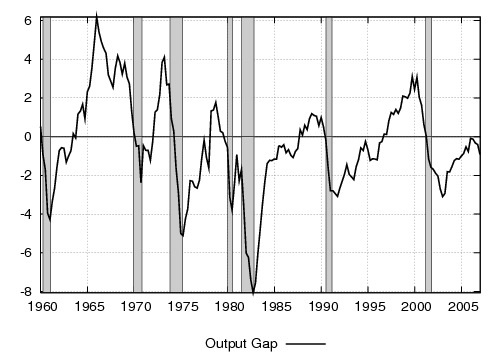
\includegraphics[scale=0.5]{results_re/output.png} \\ \\
\textbf{Inflation} \\ 
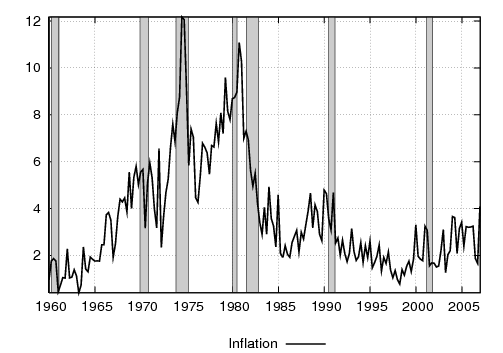
\includegraphics[scale=0.5]{results_re/inflation.png} \\
\end{tabular}
\end{center}
\end{figure}

\begin{figure}[ht]
\caption{Smoothed Probability in Volatile State}\label{fg3:pvol}
\begin{center}
\begin{tabular}{c}
\textbf{Rational Expectations} \\  
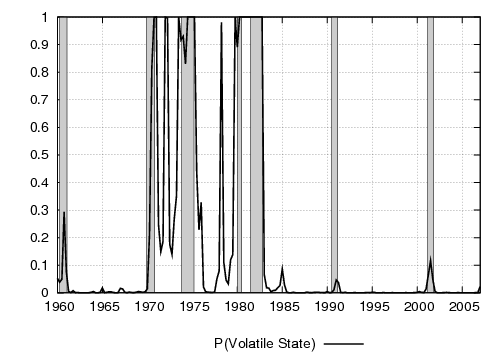
\includegraphics[scale=0.5]{results_re/states_sm.png} \\
\textbf{Dynamic Gain Learning} \\
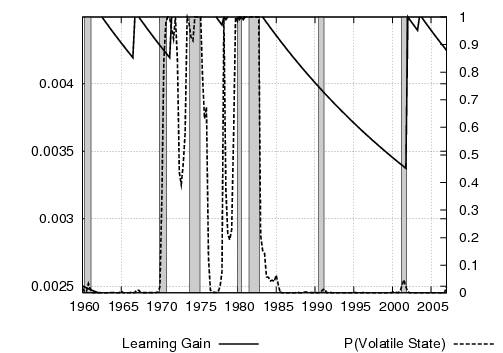
\includegraphics[scale=0.5]{results_dg8_wlsinit/states_sm.png} \\
\textbf{Constant Gain Learning} \\
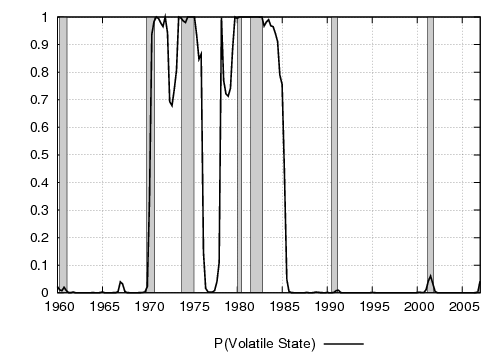
\includegraphics[scale=0.5]{results_cg_wlsinit/states_sm.png} 
\end{tabular}
\end{center}
\end{figure}

\begin{figure}[ht]
\caption{Smoothed Estimate of Natural Rate Shock}\label{fg3:natrate}
\begin{center}
\begin{tabular}{c}
\textbf{Rational Expectations} \\  
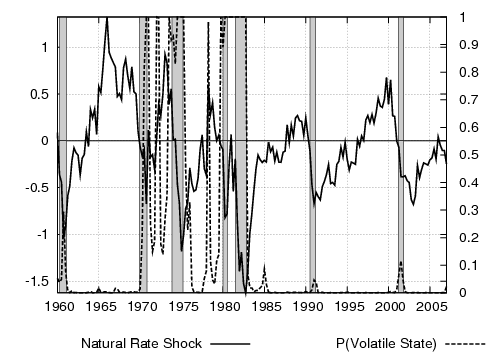
\includegraphics[scale=0.5]{results_re/natrate.png} \\
\textbf{Dynamic Gain Learning} \\
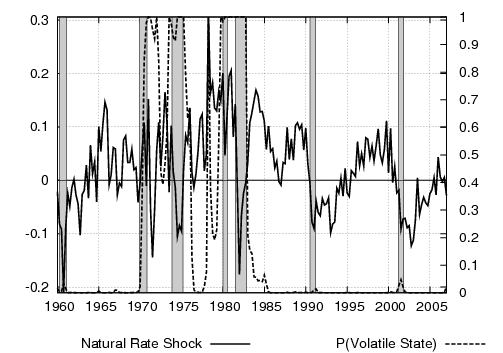
\includegraphics[scale=0.5]{results_dg8_wlsinit/natrate.png} \\
\textbf{Constant Gain Learning} \\
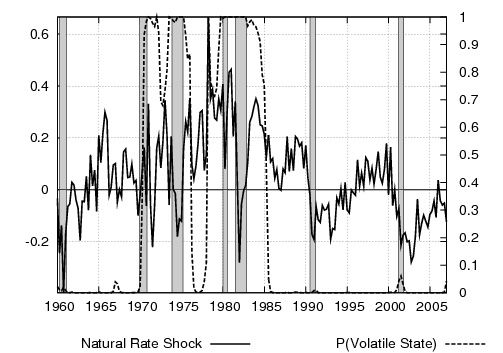
\includegraphics[scale=0.5]{results_cg_wlsinit/natrate.png} 
\end{tabular}
\end{center}
\end{figure}

\begin{figure}[ht]
\caption{Smoothed Estimate of Cost Push Shock}\label{fg3:costpush}
\begin{center}
\begin{tabular}{c}
\textbf{Rational Expectations} \\  
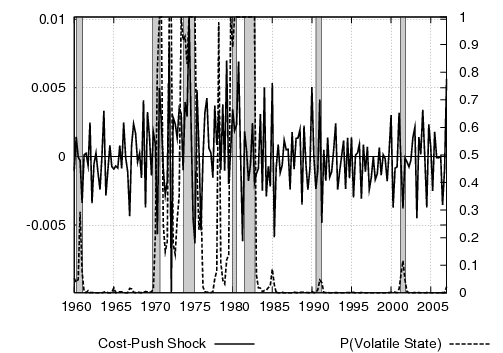
\includegraphics[scale=0.5]{results_re/costpush.png} \\
\textbf{Dynamic Gain Learning} \\
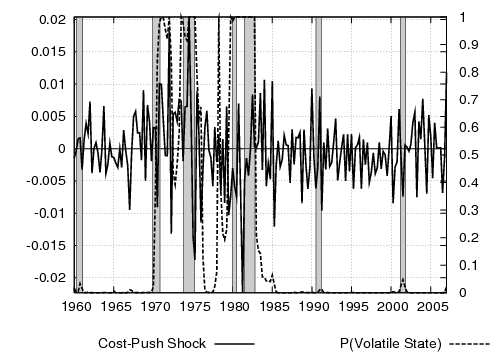
\includegraphics[scale=0.5]{results_dg8_wlsinit/costpush.png} \\
\textbf{Constant Gain Learning} \\
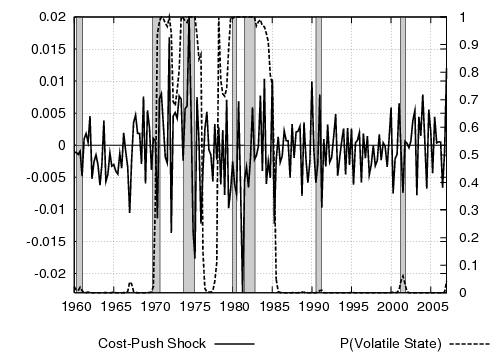
\includegraphics[scale=0.5]{results_cg_wlsinit/costpush.png} 
\end{tabular}
\end{center}
\end{figure}

\begin{figure}[ht]
\caption{Smoothed Estimate of Monetary Policy Shock}\label{fg3:mpshock}
\begin{center}
\begin{tabular}{c}
\textbf{Rational Expectations} \\  
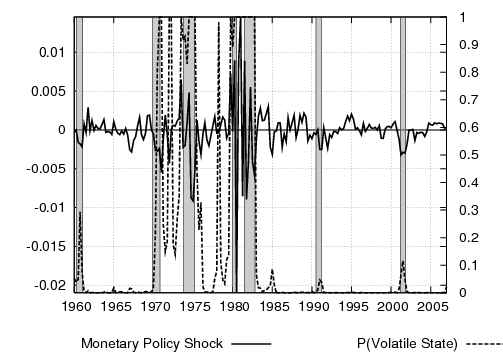
\includegraphics[scale=0.5]{results_re/mpshock.png} \\
\textbf{Dynamic Gain Learning} \\
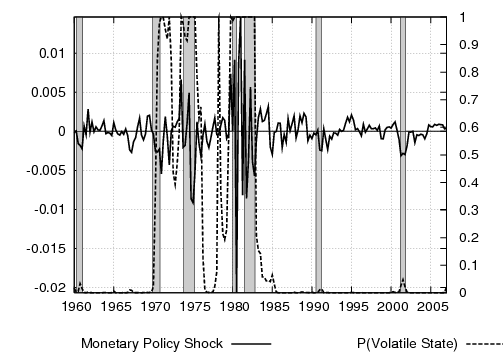
\includegraphics[scale=0.5]{results_dg8_wlsinit/mpshock.png} \\
\textbf{Constant Gain Learning} \\
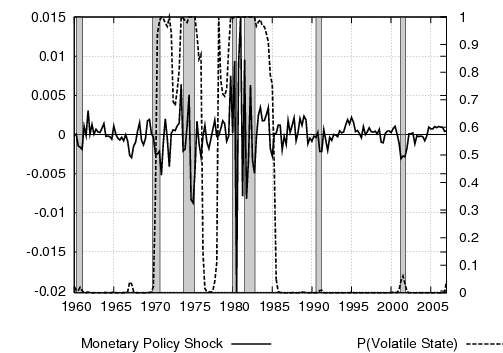
\includegraphics[scale=0.5]{results_cg_wlsinit/mpshock.png} 
\end{tabular}
\end{center}
\end{figure}

\begin{figure}[ht]
\caption{Agents' Expectations}\label{fg3:exp}
\begin{center}
\begin{tabular}{cc}
\multicolumn{2}{c}{\textbf{Dynamic Gain Learning}} \\
Output Gap & Inflation \\
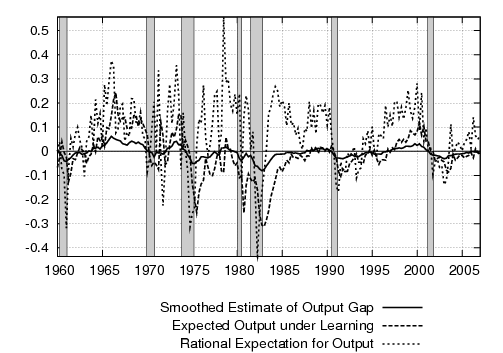
\includegraphics[scale=0.4]{results_dg8_wlsinit/output_expre.png} & 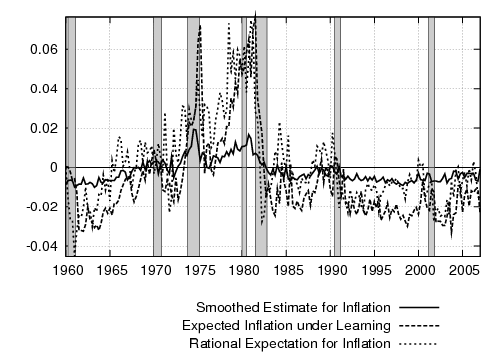
\includegraphics[scale=0.4]{results_dg8_wlsinit/inflation_expre.png} \\\\
\multicolumn{2}{c}{\textbf{Constant Gain Learning}} \\
Output Gap & Inflation \\
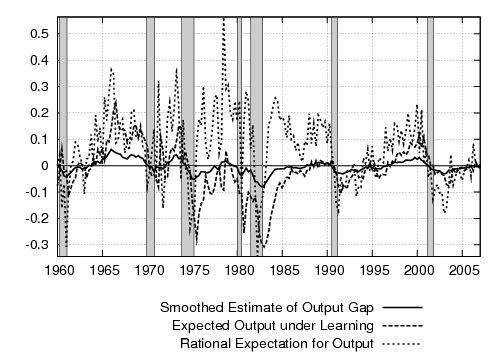
\includegraphics[scale=0.4]{results_cg_wlsinit/output_expre.png} & 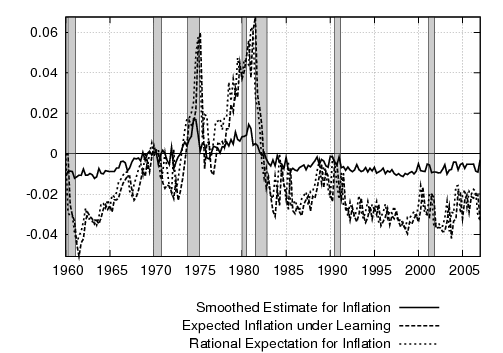
\includegraphics[scale=0.4]{results_cg_wlsinit/inflation_expre.png} \\
\end{tabular}
\end{center}
\end{figure}

\begin{figure}[ht]
\caption{One Period Ahead Output Forecast Error}\label{fg3:outputerr}
\begin{center}
\begin{tabular}{c}
\textbf{Rational Expectations} \\  
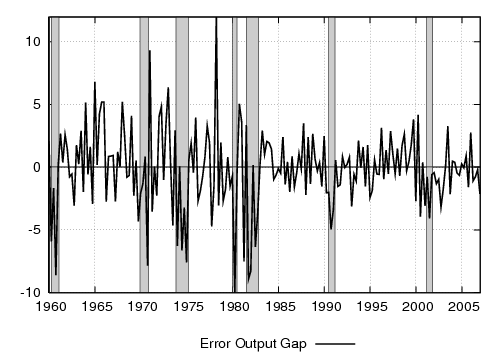
\includegraphics[scale=0.5]{results_re/output_err.png} \\
\textbf{Dynamic Gain Learning} \\
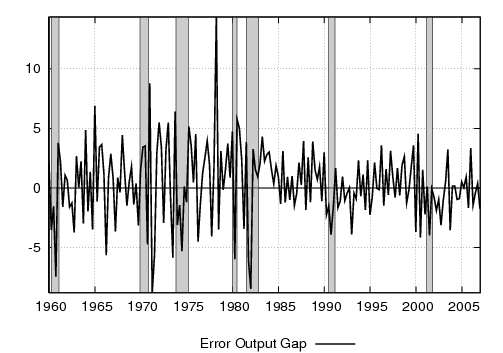
\includegraphics[scale=0.5]{results_dg8_wlsinit/output_err.png} \\
\textbf{Constant Gain Learning} \\
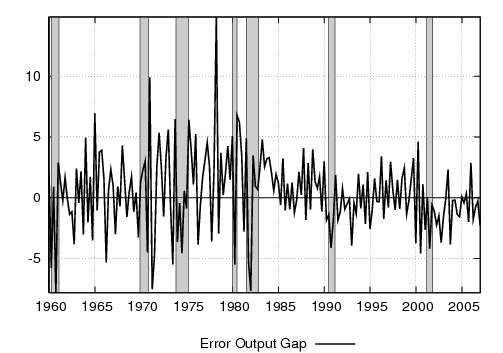
\includegraphics[scale=0.5]{results_cg_wlsinit/output_err.png} 
\end{tabular}
\end{center}
\end{figure}

\begin{figure}[ht]
\caption{One Period Ahead Inflation Forecast Error}\label{fg3:inflationerr}
\begin{center}
\begin{tabular}{c}
\textbf{Rational Expectations} \\  
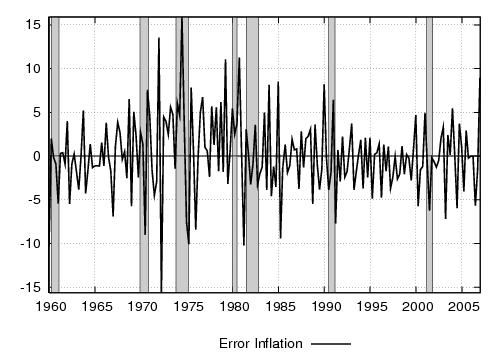
\includegraphics[scale=0.5]{results_re/inflation_err.png} \\
\textbf{Dynamic Gain Learning} \\
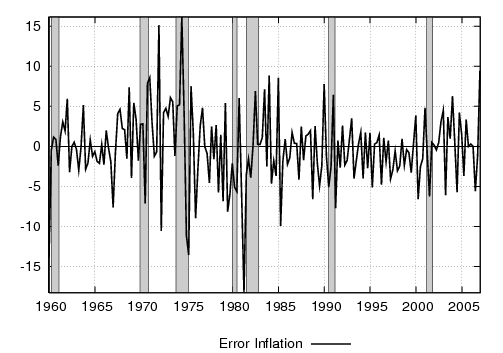
\includegraphics[scale=0.5]{results_dg8_wlsinit/inflation_err.png} \\
\textbf{Constant Gain Learning} \\
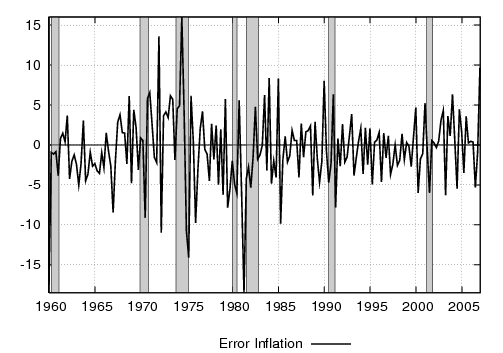
\includegraphics[scale=0.5]{results_cg_wlsinit/inflation_err.png} 
\end{tabular}
\end{center}
\end{figure}

\begin{figure}[ht]
\caption{One Period Ahead Federal Funds Rate Forecast Error}\label{fg3:fedfundserr}
\begin{center}
\begin{tabular}{c}
\textbf{Rational Expectations} \\  
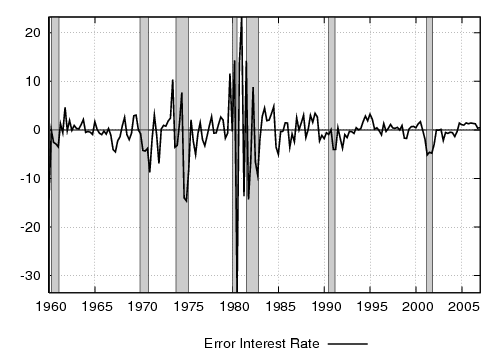
\includegraphics[scale=0.5]{results_re/fedfunds_err.png} \\
\textbf{Dynamic Gain Learning} \\
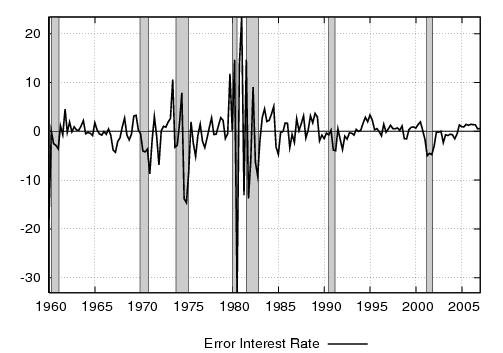
\includegraphics[scale=0.5]{results_dg8_wlsinit/fedfunds_err.png} \\
\textbf{Constant Gain Learning} \\
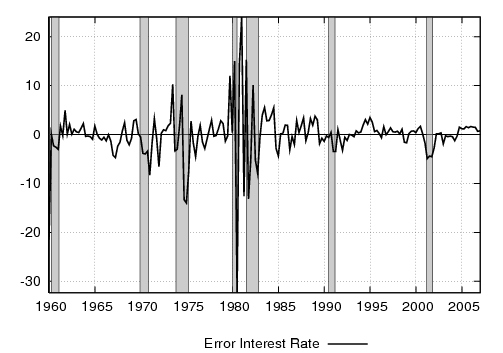
\includegraphics[scale=0.5]{results_cg_wlsinit/fedfunds_err.png} 
\end{tabular}
\end{center}
\end{figure}


\end{document}



